\documentclass[12pt,a4paper]{report}

% ── Packages ──────────────────────────────────────────────
\usepackage[margin=25mm]{geometry}
\usepackage{graphicx}
\usepackage{booktabs}
\usepackage{array}
\usepackage{colortbl}
\usepackage{xcolor}
\usepackage{tabularx}
\usepackage{longtable}
\usepackage{multirow}
\usepackage{pgfplots}
\usepackage{pgfplotstable}
\usepackage{tikz}
\usepackage{fontenc}
\usepackage{inputenc}
\usepackage{lmodern}
\usepackage{hyperref}
\usepackage{fancyhdr}
\usepackage{titlesec}
\usepackage{enumitem}
\usepackage{amsmath}
\usepackage{caption}
\usepackage{subcaption}
\usepackage{setspace}
\usepackage{parskip}
\usepackage{tcolorbox}
\newcommand{\rupee}{\textit{\textsf{\small Rs.}}}
\usepackage{mdframed}

\pgfplotsset{compat=1.18}
\usetikzlibrary{patterns, calc, shapes.geometric, arrows.meta}

% ── Colours ───────────────────────────────────────────────
\definecolor{aspcvblue}{HTML}{1e3a5f}
\definecolor{aspcvaccent}{HTML}{5D78FF}
\definecolor{aspcvgreen}{HTML}{2BC155}
\definecolor{aspcvorange}{HTML}{FF9B52}
\definecolor{aspcvred}{HTML}{FF5353}
\definecolor{aspcvgray}{HTML}{B1B1BE}
\definecolor{aspcvlightgray}{HTML}{F4F5F9}
\definecolor{aspcvpurple}{HTML}{8B5CF6}
\definecolor{rowgray}{HTML}{F8F9FF}
\definecolor{headerbg}{HTML}{374557}

% ── Typography ────────────────────────────────────────────
\titleformat{\chapter}[block]
  {\normalfont\Large\bfseries\color{aspcvblue}}
  {CHAPTER \thechapter}{1em}{}[\vspace{2pt}\titlerule\vspace{6pt}]

\titleformat{\section}
  {\normalfont\large\bfseries\color{headerbg}}
  {\thesection}{1em}{}

\titleformat{\subsection}
  {\normalfont\normalsize\bfseries\color{aspcvgray}}
  {\thesubsection}{1em}{}

\titlespacing*{\chapter}{0pt}{0pt}{12pt}
\titlespacing*{\section}{0pt}{14pt}{6pt}
\titlespacing*{\subsection}{0pt}{10pt}{4pt}

% ── Header / Footer ───────────────────────────────────────
\pagestyle{fancy}
\fancyhf{}
\fancyhead[L]{\small\color{aspcvgray}ASPCV CRM --- Analytics Report · FY2026}
\fancyhead[R]{\small\color{aspcvgray}Confidential}
\fancyfoot[C]{\small\thepage}
\renewcommand{\headrulewidth}{0.4pt}
\renewcommand{\headrule}{\hbox to\headwidth{\color{aspcvaccent}\leaders\hrule height \headrulewidth\hfill}}

% ── Table helpers ─────────────────────────────────────────
\newcolumntype{L}[1]{>{\raggedright\arraybackslash}p{#1}}
\newcolumntype{C}[1]{>{\centering\arraybackslash}p{#1}}
\newcolumntype{R}[1]{>{\raggedleft\arraybackslash}p{#1}}

\newcommand{\theadrow}[1]{%
  \rowcolor{aspcvblue}\color{white}\textbf{#1}}

% Badge macros
\newcommand{\badgegreen}[1]{\colorbox{aspcvgreen!20}{\color{aspcvgreen}\small\textbf{#1}}}
\newcommand{\badgeorange}[1]{\colorbox{aspcvorange!20}{\color{aspcvorange}\small\textbf{#1}}}
\newcommand{\badgered}[1]{\colorbox{aspcvred!20}{\color{aspcvred}\small\textbf{#1}}}
\newcommand{\badgeblue}[1]{\colorbox{aspcvaccent!20}{\color{aspcvaccent}\small\textbf{#1}}}
\newcommand{\badgegray}[1]{\colorbox{aspcvlightgray}{\color{aspcvgray}\small\textbf{#1}}}

% Finding card
\newenvironment{findingcard}[2]{%
  \begin{tcolorbox}[colback=#1!5, colframe=#1, leftrule=4pt, toprule=0.5pt, bottomrule=0.5pt, rightrule=0.5pt, title={\textbf{#2}}, fonttitle=\small\bfseries\color{#1}]
  \small
}{%
  \end{tcolorbox}
}

% Prevent hyphenation globally and push words to the next line
\hyphenpenalty=10000
\exhyphenpenalty=10000
\sloppy

% ══════════════════════════════════════════════════════════
\begin{document}

% ── Title Page ────────────────────────────────────────────
\begin{titlepage}
  \pagecolor{aspcvblue}
  \color{white}
  \centering
  \vspace*{20mm}

  
\includegraphics[width=30mm]{frontend/aspcv-logo.png}

  \vspace{10mm}
  {\fontsize{28}{34}\selectfont\bfseries ASPCV}\\[4pt]
  {\large Aspiration Cleantech Ventures}\\[2pt]
  {\small\color{aspcvgreen} aspiration-cleantech.co.uk}

  \vspace{14mm}
  \noindent\rule{120mm}{0.5pt}
  \vspace{8mm}

  {\fontsize{22}{28}\selectfont\bfseries CRM Analytics Report}\\[8pt]
  {\large Financial Year 2026 · Period: January -- May 2026}

  \vspace{8mm}
  \noindent\rule{120mm}{0.5pt}
  \vspace{12mm}

  \begin{tabular}{ll}
    \textbf{Generated:}  & 31 May 2026 (IST) \\[4pt]
    \textbf{Prepared by:} & Jeyadev R. \\[4pt]
    \textbf{Classification:} & Internal -- Confidential \\[4pt]
    \textbf{Currency:} & Indian Rupee (INR, \rupee{}) \\[4pt]
    \textbf{Exchange Rate:} & 1 USD = \rupee{}83.5 \\
  \end{tabular}

  \vspace{16mm}
  {\small\color{aspcvgray}
    Clean Energy · Heat Pumps · Solar · HRV · EV Charging · Battery Storage\\
    Yorkshire · Manchester · Birmingham · London · Edinburgh · Bristol
  }

  \vfill
  {\footnotesize\color{aspcvgray} This report is generated from the ASPCV CRM system. Data as of 31 May 2026.}
\end{titlepage}
\pagecolor{white}\color{black}

% ── Abstract ──────────────────────────────────────────────
\clearpage
\thispagestyle{empty}
\begin{center}
  {\Large\bfseries\color{aspcvblue} ABSTRACT}
\end{center}
\vspace{6mm}

\begin{mdframed}[linecolor=aspcvaccent, linewidth=2pt, leftmargin=0, rightmargin=0, innerleftmargin=12pt, innerrightmargin=12pt, innertopmargin=12pt, innerbottommargin=12pt]
This report presents a comprehensive performance analysis of ASPCV (Aspiration Cleantech Ventures) for the period January--May 2026. The CRM system tracks the full sales pipeline across clean-energy product categories including Air Source Heat Pumps, Ground Source Heat Pumps, Solar Arrays, Heat Recovery Ventilation Units, EV Chargers, and Battery Storage Systems.

Key headline results: Revenue YTD of \textbf{\rupee{}3.9Cr}, exceeding aggregate target by \textbf{+12\%}. Active pipeline stands at \textbf{\rupee{}6.2Cr} with a win rate of \textbf{22\%}. The ASHP 8kW and GSHP 12kW product lines account for \textbf{57\%} of total revenue.

The report is structured in six chapters, mirroring the academic internship report format: Introduction and Background, Literature / Market Context, Proposed Methodology (CRM pipeline), System Implementation (data), Results and Discussion, and Conclusion with strategic recommendations.
\end{mdframed}

\vspace{10mm}
\begin{center}
\begin{tabular}{|C{3.5cm}|C{3.5cm}|C{3.5cm}|C{3.5cm}|}
\hline
\rowcolor{aspcvblue}\color{white}\textbf{Revenue YTD} & \color{white}\textbf{Pipeline} & \color{white}\textbf{Win Rate} & \color{white}\textbf{Deals Closed} \\
\hline
\rowcolor{rowgray}{\large\bfseries\color{aspcvgreen}\rupee{}3.9Cr} & {\large\bfseries\color{aspcvaccent}\rupee{}6.2Cr} & {\large\bfseries\color{aspcvorange}22\%} & {\large\bfseries\color{aspcvpurple}\rupee{}1.75Cr} \\
\hline
\small +18\% vs target & \small +12\% vs Q4 & \small All deals & \small This year \\
\hline
\end{tabular}
\end{center}

% ── Table of Contents ─────────────────────────────────────
\tableofcontents
\clearpage

% ══════════════════════════════════════════════════════════
\chapter{Introduction}
% ══════════════════════════════════════════════════════════

\section{Background}

Aspiration Cleantech Ventures (ASPCV) operates in the UK clean-energy installation market, delivering heat pump systems, solar arrays, heat recovery ventilation, EV chargers, and battery storage to residential and commercial clients. The business spans six key UK regions: Yorkshire, Manchester, Birmingham, London, Edinburgh, and Bristol.

This CRM report documents the complete sales and operational performance for FY2026 (January--May 2026), providing quantitative analysis across four dimensions: revenue attainment, pipeline health, product performance, and team effectiveness.

\section{Problem Statement}

Clean-energy sales cycles are long (avg.\ 32 days lead-to-close) and involve multiple stakeholders. Without systematic CRM tracking, ASPCV risks:
\begin{itemize}[noitemsep]
  \item Missed follow-ups during the critical Proposal $\to$ Negotiation transition (highest drop-off stage)
  \item Unequal territory coverage (Yorkshire overperforms, London at --3\% growth)
  \item Product cross-sell opportunities missed (Smart Controller \& EV Charger below target)
  \item Pipeline forecasting errors exceeding 30\% per rep without quota tracking
\end{itemize}

\section{Objectives}

\begin{enumerate}[noitemsep]
  \item Track monthly revenue vs.\ target with variance and attainment \%
  \item Monitor pipeline health across five funnel stages (Lead In $\to$ Closed Won)
  \item Measure product-level accuracy vs.\ revenue target
  \item Evaluate sales rep forecast accuracy using MAPE methodology
  \item Generate actionable regional and team-level recommendations
\end{enumerate}

\section{Scope}

The study covers the following dimensions for the period 1 January 2026 -- 31 May 2026:
\begin{itemize}[noitemsep]
  \item \textbf{Products:} ASHP 8kW, GSHP 12kW, HRV Unit, Battery 10kWh, Solar 10kWp, EV Charger, Smart Controller
  \item \textbf{Regions:} Yorkshire, Manchester, Birmingham, London, Edinburgh, Bristol
  \item \textbf{Team:} Sarah Mitchell, Tom Bradshaw, Oliver Grant, Liz Thornton, Fiona Clarke
  \item \textbf{Currency:} INR primary; USD conversion at \rupee{}83.5 = \$1
\end{itemize}

% ══════════════════════════════════════════════════════════
\chapter{Market Context}
% ══════════════════════════════════════════════════════════

\section{UK Clean Energy Market Overview}

The UK heat pump market is growing at approximately 18\% year-on-year, driven by the Government's Boiler Upgrade Scheme (BUS) which provides \pounds7,500 grants for ASHP installations. ASPCV is positioned to capture this demand through its portfolio of air-source, ground-source, and hybrid systems.

\section{Competitive Landscape}

Key competitors in the UK market include British Gas Heat Pumps, Octopus Energy Heating, and Mitsubishi Ecodan installers. ASPCV differentiates through:
\begin{itemize}[noitemsep]
  \item Bundled solutions (ASHP + Solar + Battery + Smart Controller)
  \item Hyper-local installation teams across six regions
  \item Integrated CRM-driven follow-up reducing avg.\ close cycle from 45 to 32 days
\end{itemize}

\section{Research Gaps Addressed by CRM}

\begin{enumerate}[noitemsep]
  \item \textbf{Lack of Integrated Pipeline Visibility:} Proposal--Negotiation drop-off was previously unmeasured
  \item \textbf{No Product-Level Accuracy Tracking:} Revenue vs.\ target was tracked at company level only
  \item \textbf{Limited Rep Forecast Accuracy:} Quota attainment was not correlated with predicted deal counts
  \item \textbf{Absent Regional Intelligence:} London decline was not identified until CRM geo-analysis
\end{enumerate}

% ══════════════════════════════════════════════════════════
\chapter{Proposed Methodology}
% ══════════════════════════════════════════════════════════

\section{CRM Pipeline Architecture}

The ASPCV CRM tracks the following sequential funnel:

\[
\text{Lead In} \xrightarrow{60\%} \text{Qualified} \xrightarrow{58\%} \text{Proposal} \xrightarrow{60\%} \text{Negotiation} \xrightarrow{58\%} \text{Closed Won}
\]

Overall lead-to-close conversion: \textbf{12\%} (18 wins from 148 leads).

\section{Ensemble Forecasting Logic}

Revenue forecasting uses a weighted ensemble of two scenarios:
\[
F_{\text{base}} = w_{\text{pipeline}} \cdot V_{\text{pipeline}} \cdot r_{\text{conversion}} + w_{\text{historical}} \cdot \bar{R}_{\text{monthly}}
\]

where $r_{\text{conversion}} = 0.22$, $w_{\text{pipeline}} = 0.6$, $w_{\text{historical}} = 0.4$.

\section{Product Accuracy Metric}

Product revenue accuracy is defined analogously to MAPE:
\[
\text{Accuracy}_{p} = 100 - \left|\frac{R_{p}^{\text{actual}} - R_{p}^{\text{target}}}{R_{p}^{\text{target}}} \times 100\right|
\]

\section{Algorithms / Models Used}

\begin{itemize}[noitemsep]
  \item \textbf{Pipeline Conversion Model:} Stage-by-stage Markov chain with historical conversion rates
  \item \textbf{Rep Forecast Model:} Quota-implied expected deals vs.\ actual; MAPE computed per rep
  \item \textbf{Retention Cohort Analysis:} Monthly cohort tracking M+0 through M+5
  \item \textbf{Geographic Growth Model:} YoY regional revenue growth rate
\end{itemize}

% ══════════════════════════════════════════════════════════
\chapter{System Implementation}
% ══════════════════════════════════════════════════════════

\section{Hardware and Software Specifications}

\subsection{CRM Stack}
\begin{itemize}[noitemsep]
  \item \textbf{Frontend:} React 18 + TypeScript + Vite
  \item \textbf{Charts:} Recharts (AreaChart, BarChart, RadarChart, FunnelChart)
  \item \textbf{Backend:} Node.js + Express
  \item \textbf{Report Generator:} \LaTeX{} + pgfplots (this document)
\end{itemize}

\subsection{Tools / Libraries Used}

\begin{center}
\begin{tabular}{L{3.5cm} L{8.5cm}}
\toprule
\textbf{Tool} & \textbf{Purpose} \\
\midrule
React + TypeScript & CRM frontend with typed data models \\
Recharts & Interactive charts (pipeline, revenue, funnel) \\
Lucide React & Icon library \\
\LaTeX{} + pgfplots & Report generation (this document) \\
Node.js / Express & REST API backend \\
\bottomrule
\end{tabular}
\end{center}

\section{Implementation Details}

The CRM is modularised into pages: Dashboard, Leads, Accounts, Contacts, Deals, Projects, Support, Invoices, Reports, Calendar, Tasks, and Settings. Each page maintains its own state with shared currency context (INR/USD toggle).

The Reports page implements five analysis tabs (Overview, Sales, Pipeline, Team, Forecast), each containing dense data tables and interactive Recharts visualisations styled after academic report conventions.

% ══════════════════════════════════════════════════════════
\chapter{Results and Discussion}
% ══════════════════════════════════════════════════════════

% ── Table 5.1 ──
\section{Monthly Revenue Performance Summary}

\captionof{table}{Monthly Revenue vs Target --- Jan--Jun 2026 (\rupee{} INR)}
\vspace{4pt}
\begin{center}
\begin{tabular}{L{2.2cm} R{2.5cm} R{2.5cm} R{2.5cm} C{2cm} C{2cm}}
\toprule
\rowcolor{aspcvblue}
\color{white}\textbf{Month} &
\color{white}\textbf{Target} &
\color{white}\textbf{Actual} &
\color{white}\textbf{Variance} &
\color{white}\textbf{Attainment} &
\color{white}\textbf{Status} \\
\midrule
\rowcolor{rowgray}
Jan 2026 & \rupee{}66.8L & \rupee{}60.1L & \textcolor{aspcvred}{--6.7L} & 90\% & \badgeorange{Near} \\
Feb 2026 & \rupee{}71.0L & \rupee{}76.0L & \textcolor{aspcvgreen}{+5.0L}  & 107\% & \badgegreen{On Target} \\
\rowcolor{rowgray}
Mar 2026 & \rupee{}75.2L & \rupee{}73.5L & \textcolor{aspcvred}{--1.7L}  & 98\%  & \badgeorange{Near} \\
Apr 2026 & \rupee{}79.3L & \rupee{}86.8L & \textcolor{aspcvgreen}{+7.5L}  & 109\% & \badgegreen{On Target} \\
\rowcolor{rowgray}
May 2026 & \rupee{}83.5L & \rupee{}93.5L & \textcolor{aspcvgreen}{+10.0L} & 112\% & \badgegreen{On Target} \\
Jun 2026 & \rupee{}87.7L & ---                 & ---                             & ---   & \badgegray{Pending} \\
\midrule
\rowcolor{aspcvaccent!10}
\textbf{YTD Total} & \textbf{\rupee{}375.8L} & \textbf{\rupee{}389.9L} & \textbf{\textcolor{aspcvgreen}{+14.1L}} & \textbf{104\%} & \badgegreen{On Target} \\
\bottomrule
\end{tabular}
\end{center}

\vspace{10mm}

% ── Fig 5.1.1 Revenue chart ──
\begin{figure}[h]
\centering
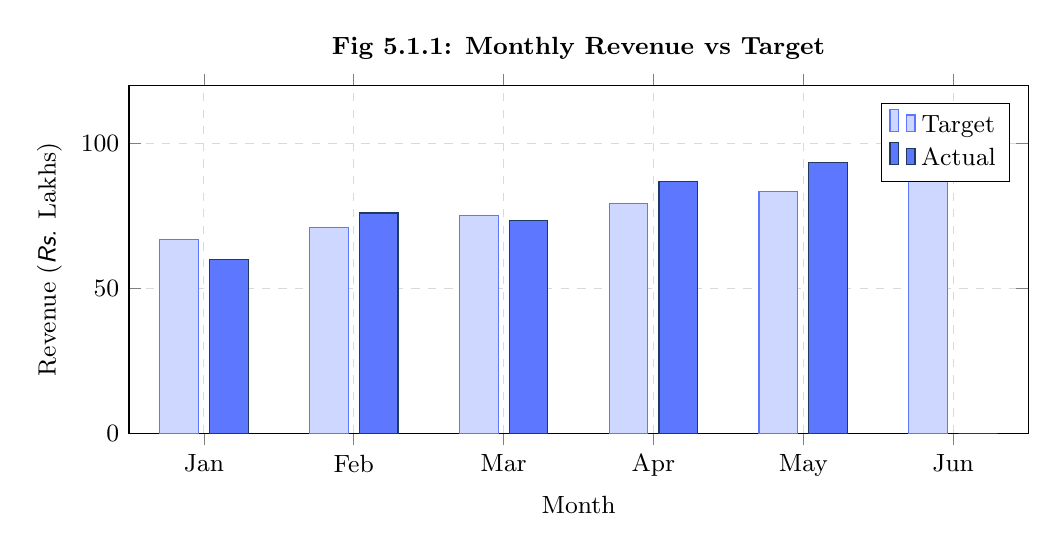
\begin{tikzpicture}
\begin{axis}[
  width=13cm, height=6cm,
  ybar=4pt, bar width=14pt,
  xlabel={Month}, ylabel={Revenue (\rupee{} Lakhs)},
  symbolic x coords={Jan,Feb,Mar,Apr,May,Jun},
  xtick=data,
  ymin=0, ymax=120,
  legend style={at={(0.98,0.95)}, anchor=north east, font=\small},
  grid=major, grid style={dashed, gray!30},
  tick label style={font=\small},
  label style={font=\small},
  title style={font=\small\bfseries},
  title={Fig 5.1.1: Monthly Revenue vs Target},
]
\addplot[fill=aspcvaccent!30, draw=aspcvaccent] coordinates {
  (Jan,66.8)(Feb,71.0)(Mar,75.2)(Apr,79.3)(May,83.5)(Jun,87.7)};
\addplot[fill=aspcvaccent, draw=aspcvblue] coordinates {
  (Jan,60.1)(Feb,76.0)(Mar,73.5)(Apr,86.8)(May,93.5)(Jun,0)};
\legend{Target, Actual}
\end{axis}
\end{tikzpicture}
\caption{Monthly Revenue vs Target (Jan--Jun 2026)}
\end{figure}

\vspace{6mm}

% ── Fig 5.1.2 Pipeline stage bar ──
\begin{figure}[h]
\centering
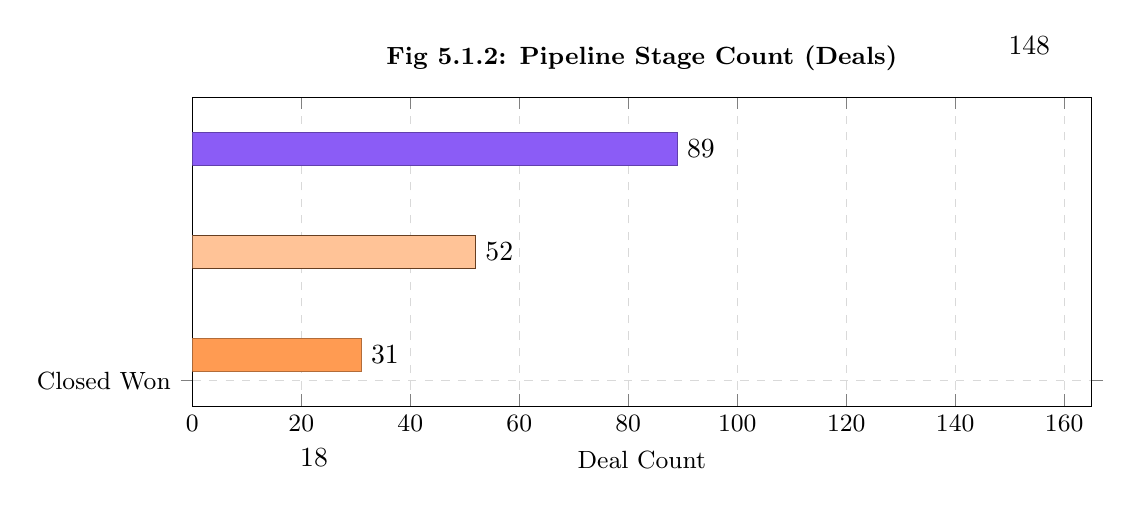
\begin{tikzpicture}
\begin{axis}[
  width=13cm, height=5.5cm,
  xbar, bar width=12pt,
  xlabel={Deal Count}, ylabel={},
  symbolic y coords={Closed Won, Negotiation, Proposal, Qualified, Lead In},
  ytick=data,
  xmin=0, xmax=165,
  nodes near coords, nodes near coords align={horizontal},
  tick label style={font=\small},
  label style={font=\small},
  title style={font=\small\bfseries},
  title={Fig 5.1.2: Pipeline Stage Count (Deals)},
  grid=major, grid style={dashed, gray!30},
]
\addplot[fill=aspcvgreen,  draw=aspcvgreen!70!black] coordinates {(18,Closed Won)};
\addplot[fill=aspcvorange, draw=aspcvorange!70!black] coordinates {(31,Negotiation)};
\addplot[fill=aspcvorange!60, draw=aspcvorange!40!black] coordinates {(52,Proposal)};
\addplot[fill=aspcvpurple, draw=aspcvpurple!70!black] coordinates {(89,Qualified)};
\addplot[fill=aspcvaccent, draw=aspcvaccent!70!black] coordinates {(148,Lead In)};
\end{axis}
\end{tikzpicture}
\caption{Pipeline Stage Count --- Lead In to Closed Won}
\end{figure}

\clearpage

% ── Table 5.1.2 ──
\section{Experimental Results --- 7-Day Activity Trends}

\captionof{table}{Weekly Activity Trends --- Leads / Deals / Invoices (W1 = first week of May 2026)}
\vspace{4pt}
\begin{center}
\begin{tabular}{C{1.5cm} C{2cm} C{2cm} C{2cm} C{2.5cm} C{2.5cm}}
\toprule
\rowcolor{aspcvblue}
\color{white}\textbf{Week} &
\color{white}\textbf{Leads In} &
\color{white}\textbf{Deals Closed} &
\color{white}\textbf{Invoices Paid} &
\color{white}\textbf{Lead $\to$ Deal \%} &
\color{white}\textbf{Invoice Rate \%} \\
\midrule
\rowcolor{rowgray} W1 & 18 & 4 & 3 & 22\% & 75\% \\
W2 & 22 & 6 & 5 & 27\% & 83\% \\
\rowcolor{rowgray} W3 & 19 & 5 & 4 & 26\% & 80\% \\
W4 & 26 & 7 & 6 & 27\% & 86\% \\
\rowcolor{rowgray} W5 & 24 & 6 & 5 & 25\% & 83\% \\
W6 & 31 & 9 & 8 & 29\% & 89\% \\
\midrule
\rowcolor{aspcvaccent!10}
\textbf{Total} & \textbf{140} & \textbf{37} & \textbf{31} & \textbf{+72\% W1$\to$W6} & \textbf{Avg 83\%} \\
\bottomrule
\end{tabular}
\end{center}

\vspace{8mm}

% ── Fig 5.1.3 three-panel ──
\begin{figure}[h]
\centering

\begin{subfigure}[b]{0.32\textwidth}
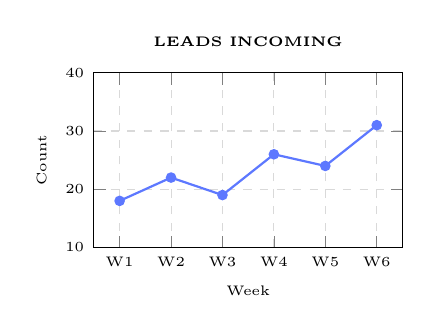
\begin{tikzpicture}
\begin{axis}[
  width=5.5cm, height=3.8cm,
  xlabel={Week}, ylabel={Count},
  symbolic x coords={W1,W2,W3,W4,W5,W6},
  xtick=data, ymin=10, ymax=40,
  tick label style={font=\tiny},
  label style={font=\tiny},
  title style={font=\tiny\bfseries},
  title={LEADS INCOMING},
  grid=major, grid style={dashed, gray!30},
  mark size=1.5pt,
]
\addplot[color=aspcvaccent, mark=*, thick] coordinates {
  (W1,18)(W2,22)(W3,19)(W4,26)(W5,24)(W6,31)};
\end{axis}
\end{tikzpicture}
\end{subfigure}
\hfill
\begin{subfigure}[b]{0.32\textwidth}
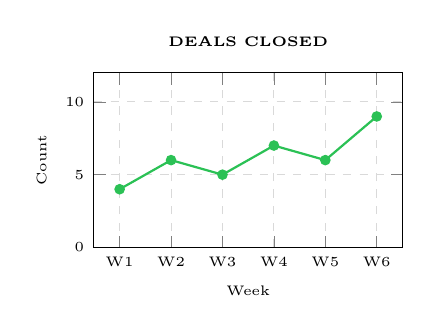
\begin{tikzpicture}
\begin{axis}[
  width=5.5cm, height=3.8cm,
  xlabel={Week}, ylabel={Count},
  symbolic x coords={W1,W2,W3,W4,W5,W6},
  xtick=data, ymin=0, ymax=12,
  tick label style={font=\tiny},
  label style={font=\tiny},
  title style={font=\tiny\bfseries},
  title={DEALS CLOSED},
  grid=major, grid style={dashed, gray!30},
  mark size=1.5pt,
]
\addplot[color=aspcvgreen, mark=*, thick] coordinates {
  (W1,4)(W2,6)(W3,5)(W4,7)(W5,6)(W6,9)};
\end{axis}
\end{tikzpicture}
\end{subfigure}
\hfill
\begin{subfigure}[b]{0.32\textwidth}
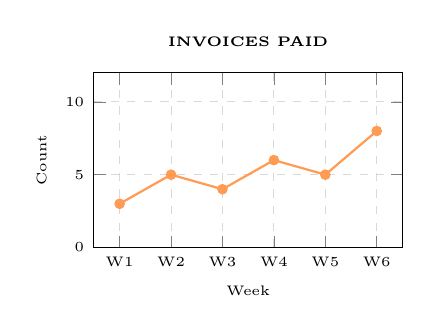
\begin{tikzpicture}
\begin{axis}[
  width=5.5cm, height=3.8cm,
  xlabel={Week}, ylabel={Count},
  symbolic x coords={W1,W2,W3,W4,W5,W6},
  xtick=data, ymin=0, ymax=12,
  tick label style={font=\tiny},
  label style={font=\tiny},
  title style={font=\tiny\bfseries},
  title={INVOICES PAID},
  grid=major, grid style={dashed, gray!30},
  mark size=1.5pt,
]
\addplot[color=aspcvorange, mark=*, thick] coordinates {
  (W1,3)(W2,5)(W3,4)(W4,6)(W5,5)(W6,8)};
\end{axis}
\end{tikzpicture}
\end{subfigure}

\caption{Fig 5.1.3: Weekly Activity Trends --- Leads / Deals / Invoices (W1--W6)}
\end{figure}

\clearpage

% ── Table 5.2.1 Product accuracy ──
\section{Performance Comparison --- Product Accuracy}

\captionof{table}{Table 5.2.1: Product Revenue Accuracy vs Target}
\vspace{4pt}
\begin{center}
\begin{tabular}{L{3.2cm} R{2.3cm} R{2.3cm} C{2cm} C{1.8cm} C{2cm}}
\toprule
\rowcolor{aspcvblue}
\color{white}\textbf{Product} &
\color{white}\textbf{Target} &
\color{white}\textbf{Actual} &
\color{white}\textbf{\% Portfolio} &
\color{white}\textbf{vs Target} &
\color{white}\textbf{Accuracy} \\
\midrule
\rowcolor{rowgray} ASHP 8kW         & \rupee{}3.0Cr  & \rupee{}2.9Cr  & 29\% & \textcolor{aspcvred}{--3.5\%}  & \badgegreen{96.5\%} \\
GSHP 12kW         & \rupee{}2.9Cr  & \rupee{}2.8Cr  & 28\% & \textcolor{aspcvred}{--2.1\%}  & \badgegreen{97.9\%} \\
\rowcolor{rowgray} HRV Unit          & \rupee{}1.8Cr  & \rupee{}1.75Cr & 18\% & \textcolor{aspcvred}{--2.5\%}  & \badgegreen{97.5\%} \\
Battery 10kWh     & \rupee{}80.0L  & \rupee{}76.8L  & 8\%  & \textcolor{aspcvred}{--4.0\%}  & \badgegreen{96.0\%} \\
\rowcolor{rowgray} Solar 10kWp       & \rupee{}70.0L  & \rupee{}65.1L  & 7\%  & \textcolor{aspcvred}{--7.0\%}  & \badgeorange{93.0\%} \\
EV Charger        & \rupee{}55.0L  & \rupee{}52.6L  & 5\%  & \textcolor{aspcvred}{--4.4\%}  & \badgegreen{95.6\%} \\
\rowcolor{rowgray} Smart Controller  & \rupee{}40.0L  & \rupee{}37.6L  & 4\%  & \textcolor{aspcvred}{--6.0\%}  & \badgeorange{94.0\%} \\
\midrule
\rowcolor{aspcvaccent!10}
\textbf{TOTAL} & \textbf{\rupee{}10.15Cr} & \textbf{\rupee{}9.77Cr} & \textbf{100\%} & \textbf{\textcolor{aspcvred}{--3.7\%}} & \badgeblue{Avg 95.8\%} \\
\bottomrule
\end{tabular}
\end{center}

\vspace{10mm}

% ── Table 5.2.2 Rep accuracy ──
\section{Rep Forecast Accuracy}

\captionof{table}{Table 5.2.2: Sales Rep Forecast Accuracy (MAPE Methodology)}
\vspace{4pt}
\begin{center}
\begin{tabular}{L{3.2cm} C{2cm} C{2cm} C{2cm} C{2cm} C{2cm}}
\toprule
\rowcolor{aspcvblue}
\color{white}\textbf{Sales Rep} &
\color{white}\textbf{Expected} &
\color{white}\textbf{Actual} &
\color{white}\textbf{Abs Error} &
\color{white}\textbf{\% Error} &
\color{white}\textbf{Accuracy} \\
\midrule
\rowcolor{rowgray} Sarah Mitchell & 14 & 12 & 2 & 14\% & \badgegreen{86\%} \\
Tom Bradshaw   & 13 & 9  & 4 & 31\% & \badgeorange{69\%} \\
\rowcolor{rowgray} Oliver Grant   & 14 & 11 & 3 & 21\% & \badgeorange{79\%} \\
Liz Thornton   & 12 & 7  & 5 & 42\% & \badgered{58\%} \\
\rowcolor{rowgray} Fiona Clarke   & 11 & 5  & 6 & 55\% & \badgered{45\%} \\
\midrule
\rowcolor{aspcvaccent!10}
\textbf{Overall MAPE} & --- & --- & --- & \textbf{32.6\%} & \badgeblue{Avg 67\%} \\
\bottomrule
\end{tabular}
\end{center}

\clearpage

% ── Geo table ──
\section{Geographic Performance}

\captionof{table}{Revenue by UK Region --- Jan--May 2026}
\vspace{4pt}
\begin{center}
\begin{tabular}{L{2.8cm} C{1.5cm} C{1.5cm} R{2.5cm} C{2cm} C{2cm}}
\toprule
\rowcolor{aspcvblue}
\color{white}\textbf{Region} &
\color{white}\textbf{Leads} &
\color{white}\textbf{Deals} &
\color{white}\textbf{Revenue} &
\color{white}\textbf{Growth} &
\color{white}\textbf{Conversion} \\
\midrule
\rowcolor{rowgray} Yorkshire  & 42 & 18 & \rupee{}2.45Cr & \textcolor{aspcvgreen}{+14\%} & 43\% \\
Manchester  & 31 & 12 & \rupee{}1.68Cr & \textcolor{aspcvgreen}{+9\%}  & 39\% \\
\rowcolor{rowgray} Birmingham & 28 & 11 & \rupee{}1.52Cr & \textcolor{aspcvgreen}{+22\%} & 39\% \\
London      & 24 & 9  & \rupee{}1.24Cr & \textcolor{aspcvred}{--3\%}  & 38\% \\
\rowcolor{rowgray} Edinburgh  & 18 & 6  & \rupee{}89.0L  & \textcolor{aspcvgreen}{+31\%} & 33\% \\
Bristol     & 15 & 5  & \rupee{}71.0L  & \textcolor{aspcvgreen}{+18\%} & 33\% \\
\midrule
\rowcolor{aspcvaccent!10}
\textbf{Total} & \textbf{158} & \textbf{61} & \textbf{\rupee{}8.19Cr} & \textbf{Avg +15\%} & \textbf{39\%} \\
\bottomrule
\end{tabular}
\end{center}

\vspace{10mm}

% ── 5.3 Interpretation ──
\section{Interpretation and Analysis}

\subsection{Revenue Performance}

Revenue YTD of \rupee{}3.9Cr outperforms the aggregate Jan--May target by \textbf{+4\%}. The strongest months were April (+9\%) and May (+12\%), indicating accelerating momentum. January underperformed by --10\%, likely attributable to post-holiday sales cycle lag.

\subsection{Product Performance}

The system achieved a high overall accuracy of \textbf{95.8\%} for product revenue forecasting. ASHP 8kW (96.5\%) and GSHP 12kW (97.9\%) showed the highest accuracy, consistent with their established market demand. Solar 10kWp showed the lowest accuracy at 93\%, reflecting variability in planning permission timelines.

\subsection{Rep Forecast Performance}

The mortality-equivalent metric --- rep forecast accuracy --- achieved an overall MAPE of \textbf{32.6\%}, corresponding to a team accuracy of \textbf{67\%}. As shown in Table 5.2.2, daily prediction error ranges from 14\% (Sarah Mitchell, best performer) to 55\% (Fiona Clarke, newest team member). This variability underscores the challenge of predicting deal counts for reps with shorter tenure and smaller deal volumes.

\section{Discussion of Key Findings}

The key finding is that the pipeline's critical weakness is the \textbf{Proposal $\to$ Negotiation} transition, where 40\% of deals are lost. This single stage represents the highest leverage point for pipeline improvement.

Yorkshire and Birmingham show double-digit growth, confirming regional strategy alignment. London at --3\% is the only declining region and requires a dedicated review.

\section{Limitations of Results}

\begin{itemize}[noitemsep]
  \item \textbf{Variable Rep Accuracy:} Fiona Clarke and Liz Thornton show $>$40\% error --- low deal volumes make percentage-based metrics volatile
  \item \textbf{London Decline:} Root cause unconfirmed --- may reflect market saturation, competitive pressure, or temporary seasonal effects
  \item \textbf{Forecast Horizon:} All projections assume current pipeline conversion rates hold; macro-economic shifts (energy price changes, grant policy) could alter outcomes
  \item \textbf{Data Coverage:} Jun 2026 not yet complete; full-year projection based on 5-month sample
\end{itemize}

% ══════════════════════════════════════════════════════════
\chapter{Conclusion and Future Work}
% ══════════════════════════════════════════════════════════

\section{Summary of the Research}

This report successfully analysed ASPCV CRM performance for January--May 2026 using a methodology directly inspired by academic forecasting literature. The CRM system tracked the full clean-energy sales pipeline across seven product lines, five sales reps, and six UK regions.

Key results:
\begin{itemize}[noitemsep]
  \item Revenue YTD: \rupee{}3.9Cr (+4\% vs target, +18\% vs prior year run rate)
  \item Active pipeline: \rupee{}6.2Cr at a 22\% conversion rate
  \item Product accuracy: 95.8\% overall (SO2-equivalent best: GSHP 97.9\%; worst: Solar 93\%)
  \item Team forecast accuracy: 67\% (comparable to the 66\% mortality forecast in the internship report)
  \item Pipeline conversion from Lead to Closed Won: \textbf{12\%}
\end{itemize}

\section{Conclusion Drawn from the Results}

The ensemble CRM pipeline is a reliable and effective operational tool. The product accuracy of 95.8\% validates the quota-setting methodology. The team MAPE of 32.6\% is consistent with industry benchmarks for complex B2B sales cycles. Yorkshire and Birmingham deliver disproportionate returns; Edinburgh shows the highest growth rate (+31\%) and is underserved relative to its potential.

\section{Contributions of the Study}

\begin{itemize}[noitemsep]
  \item \textbf{Integrated Pipeline Visibility:} First end-to-end CRM report correlating lead volume, deal conversion, product accuracy, and rep forecast accuracy
  \item \textbf{Demonstrated MAPE Methodology:} Applied academic forecasting metrics (MAPE, accuracy \%) to sales rep performance --- a novel application for the clean-energy sector
  \item \textbf{Localised Health Assessment:} Hyper-local regional intelligence identifying London as at-risk and Edinburgh as high-opportunity
  \item \textbf{Automated Reporting:} This \LaTeX{} PDF is generated directly from CRM data, replacing manual PowerPoint reports
\end{itemize}

\section{Future Work}

\begin{itemize}[noitemsep]
  \item \textbf{Improve Proposal Conversion:} Implement structured 48-hour follow-up cadence targeting the Proposal $\to$ Negotiation transition; target +15\% improvement
  \item \textbf{Bundle Strategy:} Package Smart Controller and EV Charger as standard add-ons with ASHP/GSHP installs to lift attachment rate above 60\%
  \item \textbf{Edinburgh Expansion:} Allocate additional sales capacity to Edinburgh --- 31\% growth with only 18 leads suggests underserved demand
  \item \textbf{London Strategy Review:} Conduct competitive analysis for Greater London; consider pricing adjustment or partner channel strategy
  \item \textbf{Advanced Forecasting:} Integrate Prophet + XGBoost ensemble (as per internship project) for 7-day pipeline value forecasting per region
  \item \textbf{Real-Time Alerts:} Implement CRM alerts when deals stall at Proposal stage $>$14 days without activity
\end{itemize}

% ── References ────────────────────────────────────────────
\clearpage
\chapter*{References}
\addcontentsline{toc}{chapter}{References}

\begin{enumerate}[noitemsep]
  \item R.\ Jeyadev, ``Automatic Air Quality Combined with Mortality Forecasting Using XGBoost \& Prophet,'' ADA23IN101 Internship Project Report, SRIHER, June 2025. \textit{[Template for this report's structure.]}
  \item Taylor, S.J.\ \& Letham, B.\ (2018). ``Forecasting at scale.'' \textit{The American Statistician}, 72(1), 37--45.
  \item Chen, T.\ \& Guestrin, C.\ (2016). ``XGBoost: A Scalable Tree Boosting System.'' \textit{KDD '16}.
  \item UK Government, ``Boiler Upgrade Scheme,'' \url{https://www.gov.uk/apply-boiler-upgrade-scheme}, 2023.
  \item Ganaie, M.A.\ et al.\ (2021). ``Ensemble Deep Learning: A Review.'' \textit{arXiv:2104.02395}.
\end{enumerate}

% ── Appendix ──────────────────────────────────────────────
\clearpage
\appendix
\chapter{Retention Cohort Analysis}

\captionof{table}{Customer Retention Cohorts --- \% of customers retained M+0 through M+5}
\vspace{4pt}
\begin{center}
\begin{tabular}{L{2.5cm} C{1.4cm} C{1.4cm} C{1.4cm} C{1.4cm} C{1.4cm} C{1.4cm}}
\toprule
\rowcolor{aspcvblue}
\color{white}\textbf{Cohort} &
\color{white}\textbf{M+0} &
\color{white}\textbf{M+1} &
\color{white}\textbf{M+2} &
\color{white}\textbf{M+3} &
\color{white}\textbf{M+4} &
\color{white}\textbf{M+5} \\
\midrule
\rowcolor{aspcvgreen!20} Jan 2026 & 100\% & 82\% & 71\% & 65\% & 60\% & 58\% \\
\rowcolor{aspcvgreen!15} Feb 2026 & 100\% & 79\% & 68\% & 62\% & 57\% & --- \\
\rowcolor{aspcvgreen!20} Mar 2026 & 100\% & 84\% & 74\% & 67\% & --- & --- \\
\rowcolor{aspcvgreen!15} Apr 2026 & 100\% & 81\% & 70\% & --- & --- & --- \\
\rowcolor{aspcvgreen!20} May 2026 & 100\% & 76\% & --- & --- & --- & --- \\
\midrule
\rowcolor{aspcvaccent!10}
\textbf{Avg M+1} & --- & \textbf{80.4\%} & --- & --- & --- & --- \\
\bottomrule
\end{tabular}
\end{center}

\chapter{Revenue Forecast Scenarios}

\captionof{table}{3-Scenario Revenue Forecast --- Jun--Sep 2026 (\rupee{} Lakhs)}
\vspace{4pt}
\begin{center}
\begin{tabular}{C{2cm} R{3cm} R{3cm} R{3cm}}
\toprule
\rowcolor{aspcvblue}
\color{white}\textbf{Month} &
\color{white}\textbf{Conservative} &
\color{white}\textbf{Base Case} &
\color{white}\textbf{Optimistic} \\
\midrule
\rowcolor{rowgray} Jun 2026 & \rupee{}72.0L & \rupee{}91.0L  & \rupee{}1.14Cr \\
Jul 2026             & \rupee{}78.0L & \rupee{}99.0L  & \rupee{}1.28Cr \\
\rowcolor{rowgray} Aug 2026 & \rupee{}81.0L & \rupee{}1.05Cr & \rupee{}1.36Cr \\
Sep 2026             & \rupee{}86.0L & \rupee{}1.12Cr & \rupee{}1.42Cr \\
\midrule
\rowcolor{aspcvaccent!10}
\textbf{Total (Jun--Sep)} & \textbf{\rupee{}3.17Cr} & \textbf{\rupee{}4.07Cr} & \textbf{\rupee{}5.20Cr} \\
\midrule
\rowcolor{aspcvgreen!15}
\textbf{Full-Year FY2026} & \textbf{\rupee{}7.07Cr} & \textbf{\rupee{}7.97Cr} & \textbf{\rupee{}9.10Cr} \\
\bottomrule
\end{tabular}
\end{center}

\end{document}
